%===============================================================================
%
% Main.tex
%
% Autor: Robert Gaugl
%
% Inhalt: Dieses File beinhaltet alle usepackages und Dokumenteinstellungen,
%         sowie die Aufrufe der einzelnen Unterkapitel
%
%===============================================================================


%===============================================================================
% Definition der Dokumenteigenschaften
% (A4 Papiergröße, Formeln linksbündig ausrichten, Header und Footer Linie, 
% Schriftgröße 12)
\documentclass[a4paper,fleqn,headsepline,footsepline,12pt, parskip=half]{scrartcl}
% Definiere Größe des Contentbereiches
\areaset{16cm}{27cm}

%===============================================================================
% Aufruf der verschiedenen usapackages

% Neue deutsche Silbentrennung und in Folge deutsche Begriffe wie 
% Inhaltsverzeichnis
\usepackage[ngerman]{babel}

% Um leere Seiten einzufügen
\usepackage{afterpage}
\newcommand{\blankpage}{
	\null
	\thispagestyle{empty}
	\addtocounter{page}{-1}
	\newpage}

% Mathematikpaket für zB Binimonalformeln
\usepackage[]{amsmath}

% Verhindern von 'Hurenkindern' (einzelne Zeile eines Absatzes am Anfang einer % Seite) und 'Schusterjungen' (Einzelne Zeile eines Absatzes am Ende einer Seite)
\clubpenalty = 10000
\widowpenalty = 10000
\interlinepenalty = 10000

% Definition der Zeichencodierung
\usepackage[T1]{fontenc}
\usepackage[utf8]{inputenc}

% When using babel or polyglossia with biblatex, loading csquotes is recommended 
% to ensure that quoted texts are typeset according to the rules of your main 
% language.
\usepackage{csquotes}

% Für Euro Symbol --> \euro
\usepackage{eurosym}

% chemische Abkürzungen
\usepackage[version=4]{mhchem}

% Bilder an der exakten Position darstellen
\usepackage{float}

% Zum Erstellen des Literaturverzeichnisses
\usepackage[backend = biber,
style=ieee, % Zitierstil
sorting=none, % Sortierung nach Vorkommen im Text
natbib=true, % Bereitstellen von natbib-kompatiblen Zitierkommandos
hyperref=true, % hyperref-Paket verwenden, um Links zu erstellen
maxbibnames = 3, % nur die ersten drei Autoren anzeigen 
dashed=false, % Autoren immer anzeigen
]{biblatex}
\DefineBibliographyStrings{german}{
  andothers = {et al}
}

%Vermeiden von über den Rand ragenden Links im Literaturverzeichnis
\usepackage{url}
\setcounter{biburlnumpenalty}{100}
\setcounter{biburlucpenalty}{100}
\setcounter{biburllcpenalty}{100}

% Einbinden der bib-Datei
\addbibresource{./Literatur.bib} 

% Package for adding To-Do's
\usepackage{todonotes}

% Paket für Farben im Text
\usepackage{color} 

% Pakete für Tabellen
\usepackage{colortbl} 
\usepackage{hhline} 
\usepackage{multirow} 
\usepackage{booktabs}
\usepackage{tabularx}

% Wenn Bilder eingefügt werden sollen muss das drinstehen
\usepackage{graphicx} 

% Definition des Zeilenabstandes
\usepackage[onehalfspacing]{setspace}

% Packet für Anzeige der Referenzen im PDF - Browser
\usepackage[pdfborder={0 0 0}]{hyperref}

% Einrückung von Formeln
\setlength{\mathindent}{1cm}

% Bis zu welcher Gliederungsebene soll nummeriert werden
\setcounter{secnumdepth}{5}

% Welche Ebenen sollen ins Inhaltsverzeichnis
\setcounter{tocdepth}{3}

% Prozedur zur kapitelweisen Beschriftung von Gleichungen
\makeatletter 
\@addtoreset{equation}{section} 
\renewcommand \theequation
  {\ifnum \c@section >\z@ \thesection.\fi
  \@arabic \c@equation } 
\makeatother 

% Theorem für Beispielumgebungen
\newtheorem{Beispiel}{Beispiel}[section] 

% Prozedur zur kapitelweisen Beschriftung von Bildern
\makeatletter 
\@addtoreset{figure}{section} 
\renewcommand \thefigure
  {\ifnum \c@section >\z@ \thesection.\fi
  \@arabic \c@figure } 
\makeatother 

% Prozedur zur kapitelweisen Beschriftung von Tabellen
\makeatletter 
\@addtoreset{table}{section} 
\renewcommand \thetable
  {\ifnum \c@section >\z@ \thesection.\fi
  \@arabic \c@table } 
\makeatother 

%===============================================================================
%Jetzt beginnt das eigentliche Dokument

\begin{document}
	
	%===========================================================================
	% Pre-content Seiten
	
	% Titelseite
	% !TEX root = ../Main.tex
%===============================================================================
%
% Titelseite.tex
%
% Autor: Robert Gaugl
%
% Inhalt: Titelseite des Dokuments
%
%===============================================================================

\pagestyle{empty} \enlargethispage*{23cm}
	
\vspace*{-1.5cm}
\begin{center}
	\hspace*{-1.1cm}
	
\includegraphics[width=3.3cm]{Abbildungen/TU_Graz_Logo.pdf}
			
	\vspace*{2cm}
	
	{\normalsize \textbf{\todo{Ändern}Vorname Nachname\\}}
	

	\vspace*{1.5cm} \LARGE\textbf{\todo{Ändern}Titel der Arbeit}\vspace*{1.5cm} \vfill
	
	
	\large{\textbf{\todo{Ändern für Bachelorarbeit}MASTERARBEIT\\}} \vspace*{.7cm}

	\vspace*{0.7cm}{\normalsize zur Erlangung des akademischen Grades\\}
	\vspace*{0.7cm}{\normalsize \todo{Ändern für Bachelorarbeit auf Bachelor of Science}Diplom-Ingenieur\\}

	\vspace*{1.5cm}{\normalsize eingereicht an der\\}
	\vspace*{0.7cm}\large{\textbf{Technischen Universität Graz\\}}
	
	\vspace*{1.5cm}\large{\textbf{Betreuer\\}}
	{\normalsize \todo{Ändern}Titel Vorname Nachname\\}
	\large{\textbf{Begutachter\\}} % Bei Bachelorarbeiten auskommentieren
	{\normalsize Titel Vorname Nachname\\} % Bei Bachelorarbeiten auskommentieren
	
	\vspace*{0.7cm}
	\normalsize Institut für Elektrizitätswirtschaft und Energieinnovation\\
	
	\vspace*{2cm}\small{\textbf{Graz, \todo{Ändern}November 2019\\}} \vspace*{.7cm}
	
\end{center}

\clearpage 	
	\blankpage
	
	% Ausschalten der Kopf- und Fußzeilen und Seitennummerierung auf römische 
	% Zahlen setzen
	\pagestyle{plain}
	\pagenumbering{roman}
	
	% Eidesstaatliche Erklärung
	% !TEX root = ../Main.tex
%===============================================================================
%
% Eidesstaatliche_Erklaerung.tex
%
% Autor: Robert Gaugl
%
% Inhalt: Eidesstaatliche Erklärung auf Deutsch und Englisch
%
%===============================================================================

\newcommand{\textfield}[2]
{
	\vbox
	{
		\hsize=#1\kern3cm\hrule\kern1ex
		\hbox to \hsize{\strut\hfil\footnotesize#2\hfil}
	}
}

\vspace*{\fill}
\section*{Eidesstattliche Erklärung}\vspace*{-0.7cm}
\section*{\textit{Affidavit}}

Ich erkläre an Eides statt, dass ich die vorliegende Arbeit selbstständig verfasst, andere als die angegebenen Quellen/Hilfsmittel nicht benutzt, und die den benutzten Quellen wörtlich und inhaltlich entnommenen Stellen als solche kenntlich gemacht habe. Das in TUGRAZonline hochgeladene Textdokument ist mit der vorliegenden Masterarbeit identisch \todo{Satz löschen für Bachelorarbeiten}.

\textit{I declare that I have authored this thesis independently, that I have not used other than the declared sources/resources, and that I have explicitly indicated all material which has been quoted either literally or by content from the sources used. The text document uploaded to TUGRAZonline is identical to the present master thesis.\todo{Delete sentence for Bachelorthesis}}

\hbox to \hsize{\textfield{4cm}{Datum / Date}\hfil\hfil\textfield{7cm}{Unterschrift / Signature}}
\vspace*{\fill}


 

	\newpage
	
	% Danksagung
	% !TEX root = ../Main.tex
%===============================================================================
%
% Danksagung.tex
%
% Autor: Robert Gaugl
%
% Inhalt: Danksagung
%
%===============================================================================

\section*{Danksagung}

Lorem ipsum dolor sit met, consetetur sadipscing elitr, sed diam nonumy eirmod tempor invidunt ut labore et dolore magna aliquyam erat, sed diam voluptua. At vero eos et accusam et justo duo dolores et ea rebum. Stet clita kasd gubergren, no sea takimata sanctus est Lorem ipsum dolor sit amet. Lorem ipsum dolor sit amet, consetetur sadipscing elitr, sed diam nonumy eirmod tempor invidunt ut labore et dolore magna aliquyam erat, sed diam voluptua. At vero eos et accusam et justo duo dolores et ea rebum. Stet clita kasd gubergren, no sea takimata sanctus est Lorem ipsum dolor sit amet. Lorem ipsum dolor sit amet, consetetur sadipscing elitr, sed diam nonumy eirmod tempor invidunt ut labore et dolore magna aliquyam erat, sed diam voluptua. At vero eos et accusam et justo duo dolores et ea rebum. Stet clita kasd gubergren, no sea takimata sanctus est Lorem ipsum dolor sit amet.

Duis autem vel eum iriure dolor in hendrerit in vulputate velit esse molestie consequat, vel illum dolore eu feugiat nulla facilisis at vero eros et accumsan et iusto odio dignissim qui blandit praesent luptatum zzril delenit augue duis dolore te feugait nulla facilisi. Lorem ipsum dolor sit amet, consectetuer adipiscing elit, sed diam nonummy nibh euismod tincidunt ut laoreet dolore magna aliquam erat volutpat.

Ut wisi enim ad minim veniam, quis nostrud exerci tation ullamcorper suscipit lobortis nisl ut aliquip ex ea commodo consequat. Duis autem vel eum iriure dolor in hendrerit in vulputate velit esse molestie consequat, vel illum dolore eu feugiat nulla facilisis at vero eros et accumsan et iusto odio dignissim qui blandit praesent luptatum zzril delenit augue duis dolore te feugait nulla facilisi.

Nam liber tempor cum soluta nobis eleifend option congue nihil imperdiet doming id quod mazim placerat facer possim assum. Lorem ipsum dolor sit amet, consectetuer adipiscing elit, sed diam nonummy nibh euismod tincidunt ut laoreet dolore magna aliquam erat volutpat. Ut wisi enim ad minim veniam, quis nostrud exerci tation ullamcorper suscipit lobortis nisl ut aliquip ex ea commodo consequat. 





	\newpage
	
	% Kurzfassung
	% !TEX root = ../Main.tex
%===============================================================================
%
% Kurzfassung.tex
%
% Autor: Robert Gaugl
%
% Inhalt: Kurzfassung auf Deutsch und Englisch
%
%===============================================================================

\section*{Kurzfassung}

Max. 4.000 Zeichen inkl. Leerzeichen. Unbedingt einhalten, weil die Kurzfassung im weiteren Verlauf auch ins TUGonline hochgeladen werden muss und dort diese Grenze gilt.

Eine allgemeine Zusammenfassung über den Inhalt der Arbeit. Es soll sich nicht einfach um eine Zusammenfassung aller Kapitel handeln, sondern fasse kurz die Fragestellung der Arbeit zusammen und begründe warum es eine behandlungswürdige Fragestellung ist. Erkläre kurz wie du vorgegangen bist und gib eventuell auch einen kleinen Überblick über die Resultate deiner Arbeit.

\newpage

\section*{Abstract}

Same as in chapter Kurzfassung, only in English. Also only 4.000 characters including spaces.




 

	\newpage

	% Inhaltsverzeichnis
	% !TEX root = ../Main.tex
%===============================================================================
%
% Inhaltsverzeichnis.tex
%
% Autor: Robert Gaugl
%
% Inhalt: Inhaltsverzeichnis
%
%===============================================================================

%Inhaltsverzeichnis
\tableofcontents
\pagebreak
	\newpage
	
	%===========================================================================
	% Eigentlicher Inhalt
	
	% Einschalten der Kopf- und Fußzeilen und Seitennummerierung auf arabische
	% Zahlen setzen
	\pagestyle{headings}
	\pagenumbering{arabic}
	
	% Kapitel Einleitung
	% !TEX root = ../Main.tex
%===============================================================================
%
% Einleitung.tex
%
% Autor: Robert Gaugl
%
% Inhalt: Lorem Ipsum
%
%===============================================================================

\section{Einleitung}

In diesem Kapitel soll erläutert werden, warum und wieso deine Fragestellung deiner Arbeit von Interesse ist. Außerdem können hier allgemeine Erklärungen rund um deine Arbeit beschrieben werden bzw. kann hier ein Überblick über die aktuellen Technologien gegeben werden. Ein ToDo kann mit dem Befehl \textbackslash todo\{text\} eingefügt \todo{Dies ist ein Beispiel ToDo.}werden.


\subsection{Unterkapitel}

So sieht ein Unterkapitel\footnote{In einer Fußnote können Details, welche nicht so wichtig sind um sie im Haupttext zu erklären, niedergeschrieben werden.} aus.

Um einen Zahlensalat ala {\glqq}1.2.1.3.4.5 Unterkapitel 5{\grqq} zu vermeiden, verwende wenn möglich maximal Überschriften mit drei (1.2.3 Überschrift) bis maximal vier (1.2.3.4 Überschrift) Zahlen in der Nummerierung. Im Inhaltsverzeichnis werden nur Überschriften mit drei Zahlen in der Nummerierung dargestellt.


\subsubsection{Bilder}

In Abbildung~\ref{fig:Baum} ist ein Beispiel für ein Bild mit entsprechender Bildunterschrift dargestellt. Jedes Bild muss im Text auch beschrieben und verwiesen werden. Bei nicht selbstgemachten Bildern die Quellenangabe nicht vergessen. Wenn ein Bild selber erstellt wurde, aber auf Zahlen einer anderen Quelle beruht, muss dies auch angegeben werden (Zahlen von [XY]).

\begin{figure}[H]
	\begin{center}
		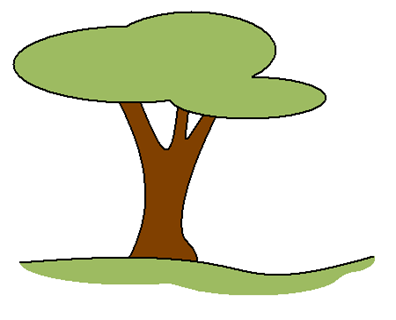
\includegraphics{Abbildungen/Baum.png}
		\caption{Das ist ein schöner Baum}
		\label{fig:Baum}
	\end{center}
\end{figure}


\subsubsection{Tabellen}

Die Gestaltung einer Tabelle obligt dem Bacheloranden/Diplomanden. Sie sollten jedoch klar leserlich und wenn möglich ein einheitliches Design im ganzen Dokument besitzen.

Sollten Tabellen aus dem Internet verwendet werden, so sollten diese selbst neu geschrieben werden und mit einer entsprechenden Quelle versehen werden. Tabelle~\ref{tab:Tabelle1} ist ein Beispiel wie eine Tabelle aussehen kann.

Bei uns am Institut gibt es keine einheitliche Regel ob die Tabellenbeschriftung oberhalb oder unterhalb der Tabelle zu stehen hat. Wie bei Abbildungen gilt allerdings: Jede Tabelle muss im Text beschrieben und verwiesen werden.

\begin{table}[H]
	\centering 
	\begin{tabular}{c c c c c}
		\hline
		\textbf{Szenarien}		& \textbf{RAV } 		& \textbf{Mehrkosten}	& \textbf{Mehrkosten}	& \textbf{Mehrkosten}	\\	
		& [\%]       			& [\euro/MWh]  			& [Mio.\euro] 			& [\euro/MWh] 			\\
		\hline
		\rowcolor[gray]{0.9}
		Szenario 1				& 0,5	 				& 5						& 0,242					& 14,9					\\
		Szenario 2				& 0,5	  				& 10					& 0,390					& 24,1					\\
		\rowcolor[gray]{0.9}
		Szenario 3				& 0,5   				& 20					& 0,692					& 42,8					\\
		Szenario 4				& 1	  					& 5						& 0,331					& 20,5					\\
		\hline \hline
	\end{tabular}
	\caption{Dies ist eine Testtabelle}\label{tab:Tabelle1}
\end{table}


\subsubsection{Formeln}

Anders als bei Abbildungen und Tabellen ist die Formelnummerierung auf der rechten Seite zu platzieren. Anders als Microsoft Word erledigt dies LaTeX allerdings automatisch.

Das Zeichen für eine Multiplikation wird durch Eingabe von '\textbackslash cdot' innerhalb der Formelumgebung erreicht. Das fälschlicherweise gern verwendete '*'-Zeichen steht für eine Faltung und nicht für eine Multiplikation!

Formel~\ref{eq:Ohmsches_Gesetz} zeigt ein Beispiel für eine korrekte Formel mit entsprechender Formelnummerierung und Erklärung der Variablen.

\begin{align}
	\label{eq:Ohmsches_Gesetz}
	U &= R \cdot I
\end{align}
\vspace*{-1cm}
\begin{table}[H]
	\begin{tabular}{@{}p{1cm}@{}p{1cm}<{\dotfill}@{}p{\dimexpr\linewidth-5cm}}
		& $U$ & Spannung in $V$  \\
		& $R$ & Widerstand in $\Omega$ \\
		& $I$ & Strom in $A$ 
	\end{tabular}
\end{table}

Die Spannung $U$ berechnet sich nach dem ohm'schen Gesetz aus der Multiplikation aus Strom $I$ und Widerstand $R$.


\subsubsection{Zahlen und Einheiten}

Die Formatierung von Zahlen muss in der ganzen Arbeit einheitlich sein. 
Üblicherweise wird in deutschen Arbeiten ein Punkt als Tausendertrennzeichen verwendet (1.000~kV), seltener auch ein gebundenes Leerzeichen (1~000~kV) welches durch eine Tilde '$\sim$' im LaTeX-Code erreicht wird. Ein gebundenes Leerzeichen verhindert, dass die Zahl aufgeteilt wird und in zwei unterschiedlichen Zeilen steht.

Als Dezimaltrennzeichen wird ein Komma verwendet (13,76~m).

Wenn Werte aus englischsprachigen Quellen kopiert werden, muss darauf geachtet werden, dass die richtigen Tausender- und Dezimaltrennzeichen verwendet werden, da im englischen Kommas als Tausendertrennzeichen und Punkte als Dezimaltrennzeichen verwendet werden. Wird die englische und deutsche Formatierung vermischt, weiß man nicht mehr ob mit 8,763 nun {\glqq}Acht Komma Sieben Sechs Drei{\grqq} oder {\glqq}Achttausendsiebenhundertdreiundsechzig{\grqq} gemeint ist.

Wird die Arbeit in Englisch verfasst, so wird als Dezimaltrennzeichen ein Punkt und als Tausendertrennzeichen bevorzugt ein gebundenes Leerzeichen (Tilde  '$\sim$') oder ein Komma verwendet.

Zwischen der Zahl und der Einheit ist wiederum ein gebundenes Leerzeichen (Tilde '$\sim$') einzufügen (10~kV), damit Zahl und Einheit nicht durch einen Zeilenumbruch getrennt werden. Außnahmen sind Prozent und Gradangaben: Diese erfolgen ohne Leerzeichen zwischen Zahl und Einheit (50\%, 10$^\circ$C).
	\newpage
	
	% Kapitel Leitfaden zum Verfassen von Abschlussarbeiten
	% !TEX root = ../Main.tex
%===============================================================================
%
% Leitfaden zum Verfassen von Abschlussarbeiten.tex
%
% Autor: TU Graz
%
% Inhalt: Lorem Ipsum
%
%===============================================================================

\section{Leitfaden zum Verfassen von Abschlussarbeiten}

\subsection{Vorgehensweise bei der Themenausarbeitung}
\label{sec: vorgehensweise bei der themenausarbeitung}

Um eine Arbeit innerhalb der geplanten Zeit erfolgreich zu Ende zu bringen, sollten einige Grundregeln befolgt werden, die effizientes Arbeiten begünstigen. Folgende prinzipielle Vorgangsweise wird dazu empfohlen.

\begin{itemize}
    \item Zu Beginn der Arbeit: Erstellung einer Gliederung (Inhaltsverzeichnis). Dadurch geben Sie sich selbst von Beginn an ein inhaltliches Grundgerüst vor, das dem strukturierten Arbeiten zugutekommt. Besprechen Sie die Gliederung der Arbeit frühzeitig mit Ihrem Betreuer durch.
    \item Den Textteil nach dieser Gliederung zunächst mit Stichwörtern, sodann zunehmend mit Text sowie Tabellen und Abbildungen versehen. Halten Sie dabei das Inhaltsverzeichnis stets aktuell.
    \item Sammlung von Unterlagen wie Literaturstellen, Entwürfen von Tabellen und Abbildungen. Notieren Sie sich hierbei die Quellen, um sich die nachträgliche Recherche zu ersparen. 
    \item Vorwegnahme der erwarteten Ergebnisse und erste Formulierung der Kurzfassung und der Schlussfolgerungen (Diskussion mit dem Betreuer).
    \item Die fertige Arbeit selbst einmal vollständig auf Druckfehler, Lesbarkeit, Stil und logischen Aufbau durchlesen. Nach Möglichkeit die Arbeit zuvor einige Tage -abliegen lassen-, da sehr schnell Betriebsblindheit auftritt! Bei Masterarbeiten: auch von einer unbeteiligten Person und/oder einem Kollegen lesen lassen.
    \item Erwarten Sie keine grammatikalische Korrektur durch den Betreuer!
\end{itemize}

\newpage

%=============================================================

\subsection{Literaturrecherche}

Ausgangspunkt einer wissenschaftlichen Arbeit ist meist eine Literaturrecherche, um sich gezielt Wissen zum gewählten Thema zu verschaffen. Im Bericht werden die Ergebnisse der Literaturrecherche vorwiegend in das Kapitel -Stand der Technik- eingearbeitet.

%\vspace{2,5mm}

Die Recherche bietet im Allgemeinen wertvolle Hinweise für die Bearbeitung der eigenen Aufgabe, auch kann dadurch die {\glqq}Neuerfindung des Rades{\grqq} vermieden werden. Unter Umständen muss dazu nicht nur der aktuelle Stand der Technik sondern bis zu den Grundlagen recherchiert werden. 

%\vspace{2,5mm}

\underline{Häufig genutzte Quellen zur Literaturrecherche}
\begin{itemize}
    \item Bibliotheken
    \begin{itemize}
        \item Bibliothek der TU Graz
        \item Bibliotheken anderer Universitäten im In- und Ausland
        \item Nationalbibliotheken
        \item etc.
    \end{itemize}
     \item Patente
    \begin{itemize}
        \item Österreichisches Patenamt
        \item {\glqq}Patentfibel{\grqq} der PVA SH GmbH
        \item worldwide.espacenet.com
        \item depatisnet.dpma.de
        \item patft1.uspto.gov
        \item google.com/patents
    \end{itemize}
    \item Wissenschaftliche Artikel und Bücher
    \begin{itemize}
        \item sciencedirect.com
        \item scholar.google.com
        \item www.semanticscholar.org
        \item link.springer.com
        \item ieeexplore.ieee.org
    \end{itemize}    
\end{itemize}

%\vspace{5mm}



\newpage

%=============================================================

\subsection{Gliederung der Arbeit}

Im Folgenden wird eine mögliche Gliederung der Arbeit vorgestellt und die einzelnen Abschnitte werden näher ausgeführt. Betont sei, dass es sich dabei nur um eine Richtschnur und nicht um starre Regeln handeln kann. 

\vspace{1mm}

\textbf{(a) Titelblatt}

\vspace{1mm}

Ein Titelblatt ist in der Dokument-Vorlage (verfügbar im Teach Center) enthalten.

\vspace{1,5mm}

\textbf{(b) Eidesstattliche Erklärung / Statutory Declaratio}

\vspace{1mm}

Eine handschriftlich unterschriebene eidesstattliche Erklärung ist erforderlich. Den Text der Vorlage entnehmen.

\vspace{1,5mm}

\textbf{(c) Kurzfassung}

\vspace{1mm}

Die Kurzfassung ist vom Text der Arbeit unabhängig und wird daher vor dem Vorwort angeordnet. Sie darf nur Stichwörter, Zahlenangaben, Argumentationen etc. enthalten, die im Text der Arbeit vorkommen.

\vspace{1mm}

Empfohlene Gliederung des Textes:
\begin{enumerate}
    \item Absatz: Kurze Einführung ins Thema (Ausgangspunkt und Aufgabenstellung)
    \item Absatz: Methode, Durchführung
    \item Absatz: Ergebnisse und Schlussfolgerungen
\end{enumerate}

Die Kurzfassung soll mit möglichst wenigen Wörtern (präzisen Formulierungen) möglichst viel vom wesentlichen Inhalt der Arbeit wiedergeben.Die Kurzfassung darf nicht mit zu vielen Zahlenwerten überfrachtet werden. 

\vspace{1mm}

\underline{Für Masterarbeiten:} Es ist naheliegend, den gleichen Text für die Erfassung im TUGonline zu verwenden. Der Text sollte maximal ca. 4.000 Zeichen umfassen.

\newpage

\textbf{(d) Abstract}

\vspace{1mm}

Es folgt die Kurzfassung in englischer Sprache (Abstract). Die freie Wiedergabe des Inhalts der deutschen Kurzfassung ist besser als eine wörtliche Übersetzung.

\vspace{1mm}

\textbf{Vorwort}

\vspace{1mm}

Das Vorwort besteht meist aus wenigen Sätzen und sollte keinesfalls mehr als eine Seite umfassen.(kein muss) Meist enthält es:

\begin{itemize}
    \item Angaben über Ort und Zeit des Entstehens der Arbeit
    \item Erwähnung der verwendeten Hilfsmittel
    \item Danksagung an Firmen und Personen von Firmen oder anderen Sponsoren, sowie an Betreuer und gegebenenfalls andere Personen, die den Anstoß zur Arbeit gegeben oder bei der Durchführung der Arbeit geholfen haben.
    \item Entstand die Arbeit im Rahmen eines geförderten Projektes, ist in der Danksagung der Fördergeber zu erwähnen (sprechen Sie den genauen Wortlaut mit Ihrem Betreuer ab!), ggf. mit Logo.
\end{itemize}

\vspace{1mm}

\textbf{(f) Inhaltsverzeichnis}

\vspace{1mm}

Wiedergabe der Gliederung der Arbeit mit Dezimalklassifikation und Seitenzahlen, nach Möglichkeit nur bis 3 Stellen der Unterkapitel. Nach den Hauptkapiteln folgen (ohne Dezimalklassifikation):

\begin{itemize}
    \item Literaturverzeichnis
    \item Anhänge, Beilagen etc.
    \item Tabellenliste, Abbildungsliste, Abkürzungsliste (optional)
\end{itemize}

\newpage

\textbf{(g) Hauptteil und Anhang}

\vspace{1mm}

Achten Sie auf eine sinnvolle Hauptgliederung (i.A. nicht mehr als 9 nummerierte Hauptkapitel), z.B.:

\begin{enumerate}
    \item Einleitung
    \item Grundlagen
    \item Stand der Technik
    \item Methodik
    \item Ergebnisse
    \item Zusammenfassung/Schlussfolgerungen
\end{enumerate}
\hspace{5mm}
Abkürzungsverzeichnis (Nomenklatur)

\vspace{1mm}

\hspace{5mm}
Abbildungsliste

\vspace{1mm}

\hspace{5mm}
Tabellenliste

\vspace{1mm}

\hspace{5mm}
Literatur

\vspace{5mm}

\underline{Einleitung}

\begin{itemize}
    \item Die Einleitung bildet in der Regel das erste Hauptkapitel.
    \item Sie soll ins Thema einführen und wird die Aufgabenstellung umfassen, nachdem vorher der Stand der Technik auf dem behandelten Gebiet kurz dargestellt wurde.
    \item Lange Einführungen ins Thema sind zu vermeiden, vor allem dann, wenn es sich um schon öfter behandelte Themen handelt.
    \item Andererseits kann bei weniger oft behandelten oder {\glqq}neuen{\grqq} Themen  eine längere, die Prinzipien und technische Lösungen sowie den Stand der Wissenschaft und Technik auf diesem Gebiet beschreibende Einführung angebracht sein. In solchen Fällen ist allerdings zu überlegen, ob dem Stand der Technik ein eigenes Hauptkapitel gewidmet werden soll.
    \item In der Einleitung soll auch die Motivation der Arbeit erläutert werden.
    \item Den Schluss der Einleitung kann z.B. eine kurze Vorschau auf die kommenden Kapitel bilden.
\end{itemize}

\newpage

\underline{Hauptkapitel}

\begin{itemize}
    \item Ein Hauptkapitel über die technisch/wissenschaftlichen Grundlagen der Arbeit kann zweckmäßig sein.
    \item Bei einer praktischen Arbeit ist es notwendig die Methodik in einem Kapitel zu beschreiben.
    \item Das Kapitel vor der Zusammenfassung soll den Resultaten der Arbeit gewidmet werden.
\end{itemize}

\vspace{5mm}

\underline{Zusammenfassung/Schlussfolgerungen}

\begin{itemize}
    \item In den Schlussfolgerungen ist es zunächst angebracht, einen kurzen Rückblick über die Aufgabenstellung und die Art und Methode der Durchführung zu geben.
    \item Dann folgt eine Zusammenfassung der wesentlichen Ergebnisse.
    \item Das Schlusskapitel stellt die Essenz der Arbeit dar und wird deben der Kurzfassung am ehesten von Außenstehenden gelesen, weswegen dieses besonders klar aufgebaut und präzise formuliert sein muss.
\end{itemize}

\vspace{5mm}

\underline{Abkürzungsverzeichnis (Nomenklatur)}

\begin{itemize}
    \item Ein Abkürzungsverzeichnis ist dann sinnvoll, wenn in der Arbeit in verschiedenen Kapiteln immer wieder die gleichen Abkürzungen/Formelzeichen verwendet werden.
    \item Es wird alphabetisch geordnet und enthält ALLE in der Arbeit vorkommenden Abkürzungen und Formelzeichen.
\end{itemize}

%\newpage

%=============================================================

\subsection{Datenablage und Sicherung}

Falls z.B. in Simulationen eine große Anzahl von Ergebnisdateien zu erwarten ist, sollte bereits vor Beginn der Arbeit mit dem Betreuer das Ablageformat und die Systematik der Dateibezeichnung geklärt werden. In der Regel sind die Dateinamen systematisch zu benennen bzw. abzulegen, um bestimmte wesentliche Versuchs-/Rechenparameter schon aus der Bezeichnung erkennen zu können. Darüber hinaus wird eine regelmäßige Sicherung der Dateien empfohlen, insbesondere der zentralen Textdatei. Überprüfen Sie rechtzeitig vor dem geplanten Drucktermin der Arbeit (bzw. immer wieder zwischendurch), ob die Erstellung einer pdf-Datei (die i. A. zum Druck verwendet wird) problemlos möglich ist, insb. die Qualität der Abbildungen und richtige Darstellung von Formeln.

\newpage
%=============================================================

\subsection{Stil und formale Kriterien}
\label{sec:stil und formale kriterien}

Grundsätzlich ist davon auszugehen, dass  wissenschaftliche Arbeiten nicht von völlig fachfremden Personen gelesen und verstanden werden müssen. Dennoch empfiehlt es sich, dem Leser das Lesen möglichst zu erleichtern, indem einige stilistische wie auch formale Kriterien erfüllt werden.

\subsubsection{Allgemeine Form der Arbeit}
\label{sec:allgemeine form der arbeit}

Bei der Formatierung der Abschlussarbeit wird dem Autor an sich freie Hand gelassen, was Form und Erscheinungsbild der Arbeit betrifft. Trotzdem gilt es einige Regeln zu beachten, die beim Verfassen wissenschaftlicher Arbeiten üblich und sinnvoll sind. 

\begin{itemize}
    \item Textverarbeitung vorzugsweise in MS Word oder in LATex. Vorlage für beides ist im Teach Center zu finden.
    \item Die Schriftgröße soll so gewählt werden, dass der Fließtext der Schriftart Times New Roman mit Schriftgröße 11 entspricht: Times New Roman Schriftgröße 11, Calibri Schriftgröße 12, Arial Schriftgröße 11 etc.
    \item Ränder: Links mindestens 25 mm; andere Ränder mindestens 20 mm (darf rechts stellenweise – z.B. bei Tabellen oder Abbildungen – geringfügig überschritten werden).
    \item Seitenzahlen: römische Zahlen bis einschließlich Inhaltsverzeichnis, arabische Zahlen beginnend mit {\glqq}1{\grqq} ab dem Text der Arbeit.
    \item Kopfzeilen mit Kapitelnummer und Kapitelnamen (vorzugsweise zentriert) erleichtern die {\glqq}Orientierung{\grqq} beim Durchblättern.
    \item Rechtschreibprüfung verwenden, wenn Sie sich aber bei einer Schreibweise unsicher sind, kann bei deutschsprachigen Arbeiten \underline{http://www.duden.de/} bzw. bei englischsprachigen Arbeiten \underline{https://www.linguee.de/} gute Dienste leisten.

\end{itemize}

\newpage

\subsubsection{Schreibstil}

\begin{itemize}
    \item I.d.R. in Vergangenheitsform schreiben
    \item Vermeiden Sie die {\glqq}Ich{\grqq}- oder {\glqq}Wir{\grqq}- oder {\glqq}man{\grqq}-Form, Verwenden Sie stattdessen nach Möglichkeit Formulierungen im Passiv
    \item Verwenden Sie nur Wörter der (deutschen) Sprache, mit deren Umgang Sie vertraut sind. Die Verwendung von Fremdwörtern kann zwar ganz nett sein, aber auch sehr peinlich, wenn sie falsch angewendet werden.
    \item Oberste Priorität beim Schreiben haben Lesbarkeit und Verständlichkeit! Schachtelsätze mit unzähligen Nebensätzen sind meist nicht angebracht.
    \item Finden Sie durch Lesen der Fachliteratur heraus, welche Fachbegriffe und Abkürzungen bzw. Symbole im von Ihnen bearbeiteten Themengebiet üblich sind und verwenden Sie bevorzugt diese. Bei Unklarheiten fragen Sie Ihren Betreuer.
    \item Verwenden Sie immer den gleichen Begriff, wenn Sie wiederholt über einen bestimmten Gegenstand, eine bestimmte Vorgehensweise, etc. schreiben.
    \item Abkürzungen mindestens einmal im Text ausschreiben und erklären. Prinzipiell sparsam mit Abkürzungen umgehen. Falls viele Abkürzungen verwendet werden, ein Abkürzungsverzeichnis einfügen.
    \item Mischen Sie nicht englische und deutsche Abkürzungen, sondern entscheiden sie sich für eine Sprache und seien Sie konsequent.
    \item Vermeiden Sie {\glqq}diffuse{\grqq} Beschreibungen wie die {\glqq}Emissionen sind recht hoch{\grqq} oder {\glqq}ziemlich hoch{\grqq}, etc.
    \item Definition von speziellen Begriffen dort, wo diese erstmals auftreten
    \item Achten Sie insgesamt auf einen logischen, systematischen Aufbau Ihrer Arbeit.
\end{itemize}

\newpage

\subsubsection{Kapitel / Absätze}

\begin{itemize}
    \item Ein Hauptkapitel soll auf einer neuen Seite beginnen
    \item Auf eine Überschrift sollte unmittelbar Text folgen
    \item Geben Sie am Beginn eines Kapitels einen kurzen Überblick über die Inhalte der folgenden Abschnitte, dieser soll als Überleitung gedacht sein und nicht als reine Aufzählung.
    \item Die Kapitelnummerierung soll sinnvoll und logisch erfolgen. In der Arbeit sollten maximal vier Überschriftsebenen (1.1.1.1) und nicht mehr als 9 Hauptkapitel verwendet werden, was im üblichen Fall ausreichend ist.
    \item Führen Sie eine Untergliederung nur dann ein, wenn mindestens zwei Elemente dieser Ebene vorkommen (3.1.1 nicht notwendig, wenn 3.1.2 nicht existiert)
    \item Absätze erleichtern oftmals die Lesbarkeit, allerdings gehören sie nur dorthin, wo auch eine Trennung von Gedanken stattfindet.
    \item Absätze sind klar erkenntlich zu machen: vorzugsweise mit Leerzeile bzw. vergrößertem Zeilenabstand.
    \item Aufzählungen mit Zeichen nach Ihrer Wahl erkenntlich machen, bei besonderer Hervorhebung auch mit kleinen lateinischen Buchstaben, kleinen römischen Ziffern oder arabischen Ziffern
    \item Kontrollieren Sie nach Abschluss aller inhaltlichen Korrekturen nochmals, dass sich zwischen Tabellen bzw. Abbildungen und ihren Über- bzw. Unterschriften kein Seitenumbruch eingeschlichen hat.
\end{itemize}

\newpage

\subsubsection{Tabellen, Abbildungen, Formeln, Querverweise}
\label{sec:tabellen, abbildungen, formeln, querverweise}

\begin{itemize}
    \item Alle Tabellen und Abbildungen sind unabhängig von einander zu nummerieren, entweder durchgehend, oder  hauptkapitelweise.
    \item Überprüfen Sie zwischendurch immer wieder, ob die Querverweise noch gültig sind.
    \item Auf alle Tabellen und Abbildungen muss zumindest einmal im Text Bezug genommen werden.
    \item Tabellen und Abbildungen nach Möglichkeit nicht größer als DIN A4.
    \item Tabellen, die über zwei oder mehrere Seiten gehen, auf der zweiten Seite kennzeichnen.
    \item Vermeiden Sie {\glqq}relative Ortsangaben{\grqq} bei Verweisen (anstelle {\glqq}in der folgenden Abbildung{\grqq} besser {\glqq}in Abbildung xy{\grqq}.
    \item Abbildungen und Tabellen sollten selbsterklärend sein, d.h. die Beschriftung sollte so ausgeführt sein, dass das Wesentliche sofort ersichtlich ist.
    \item Beschreiben Sie im Text ausführlich, was in einer Abbildung zu sehen ist und welche Schlussfolgerungen daraus gezogen werden. Gehen Sie nicht davon aus, dass der Leser die Abbildung richtig interpretiert.
    \item Unterscheiden Sie bei Erläuterungen zu Abbildungen, was tatsächlich (objektiv) ersichtlich ist, und welche Schlüsse Sie bereits daraus gezogen haben.
    \item Werden Abbildungen oder Tabellen aus anderen Veröffentlichungen übernommen, so ist das durch ein Literaturzitat am Ende der Legende bzw. der Tabellenüberschrift anzugeben, und zwar auch dann, wenn dieses Zitat im Text bereits vorkommt.
    \item Schriftgröße in Abbildungen und Tabellen ca. gleich (evtl. etwas kleiner) als Standardtext. Erfahrungsgemäß geraten die Schriftzüge besonders bei Diagrammen oft zu klein.

    \item Tabellen und Abbildungen sollen möglichst nahe bei der erstmaligen Zitierung im Text angeordnet werden (sodass der Seitenumbruch günstig liegt), und zwar in der Regel nach der Zitierung.
    \item Verwenden Sie logische Linienarten(-farben) und Symbole, falls anhand von Abbildungen Einflüsse von Parametern diskutiert werden.
    
\newpage

    \item Speziell dann, wenn zwei Abbildungen zu Vergleichszwecken (z.B. Messergebnis mit vs. ohne Dämmung) nebeneinander dargestellt sind, dann sollten diese die gleiche Achsenskalierung und Größe aufweisen.
    \item Gleichungen sollten durch an den rechten Rand (rechtsbündig) gesetzte Zahlen nummeriert werden. 
    \item Bei Querverweisen zu anderen Kapiteln (oder Abbildungen in anderen Kapiteln) auch Kurzinformation darüber geben, welche Information dort zu finden ist, z.B. {\glqq}Wie in Abschnitt 3.1 beschrieben ist, kann durch eine erhöhte Geschwindigkeit…{\grqq}.
    \item Auch auf Anhänge zumindest einmal im Hauptteil mittels Querverweis Bezug nehmen
    (z.B. {\glqq}Die in Anhang A angeführten Messergebnisse…{\grqq}).
    \item Überprüfen Sie vor der Abgabe (ausgedruckt bzw. als pdf), ob alle Abbildungen in der entsprechenden Qualität vorliegen und Formeln richtig dargestellt werden. Hier kommt es immer wieder zu Problemen.
\end{itemize}

%\newpage

\subsubsection{Formale Schreibweise}
\label{sec: formale schreibweise}

\begin{itemize}
    \item Dezimaltrennzeichen: in deutschsprachigen Arbeiten Komma (,) in englischsprachigen Arbeiten Punkt (.)!
    \item Verwenden Sie keine Tausender-Trennpunkte. Anstatt Klarheit zu bringen, führt dies oft zu Missverständnissen, wenn Tausender-Trennpunkt verwendet wird! Bei großen bzw. sehr kleinen Zahlen (mehr als 4 Stellen vor oder nach dem Komma): fixes Leerzeichen zwischen Dreiergruppen (optional)
    \item Nur signifikante Stellen hinter dem Komma anschreiben
    \item Fixes Leerzeichen (Word: Strg+Umsch+Leertaste; Anzeige als Formatierungssymbol: °, LaTeX:\raisebox{-0.8ex}{\~{}} (Tilde)) vor und nach „=“ sowie zwischen Zahl und Einheit, um zu verhindern, dass die Einheit durch einen Zeilenumbruch in die nächste Zeile rutscht bzw. im Blocksatz das Leerzeichen auseinandergezogen wird
    
\newpage

    \item Schreibweise von Einheiten
    \begin{itemize}
        \item im Fließtext: ohne Klammern
        \item bei Achsenbeschriftungen in Diagrammen: Einheit in NICHT in eckiger Klammer sondern 'in'
        \item in Kopfzeilen von Tabellen: entweder nach der Bezeichnung mit 'in', oder – vorzugsweise – eine eigene Zeile/Spalte für die Einheiten einführen.
    \end{itemize}
    
%\newpage

    \item Bei Multiplikationen von Variablen in Gleichungen verwenden Sie den mittigen, kleinen Punkt oder ein fixes Leerzeichen.
    \item Achten Sie auf richtige, eindeutige Klammernsetzung.
    \item Verwenden Sie Bindestrich für zusammengesetze Wörter und den Gedankenstrich für Denkpausen.
\end{itemize}

%\newpage



%=============================================================

\subsection{Zitate, Quellen und Referenzen}

Das Übernehmen von Inhalten aus anderen Arbeiten ist üblich und sinnvoll bei der Erstellung wissenschaftlicher Dokumente, so dass Themen nicht doppelt untersucht werden müssen. Eine eindeutige Kennzeichnung solcher übernommener Stellen ist jedoch unbedingt notwendig.

\underline{Zitate im Fließtext}
\begin{itemize}
    \item Die Übernahme einzelner Fakten oder Daten aus einer anderen Quelle sind im Anschluss des Fließtextes an den zitierten Sachverhalten mit
    \begin{itemize}
        \item Name und Jahreszahl in runder Klammer -> z.B. (Maier, 1998)
        \item oder mit Nummerierung der Zitate in eckiger Klammer -> z.B. [1]
    \end{itemize}
    zu kennzeichnen.
    \item Wenn zwei verschiedene Quellen als Zitat gleich aufscheinen (gleicher Autor und gleiches Jahr), wird dem jahr ein Kleinbuchstabe in aufsteigender Reihenfolge nachgestellt.
\end{itemize}

%\vspace{5mm}

\underline{Zitieren von Absätzen}
\begin{itemize}
    \item Wird einer Quelle ein ganzer Absatz oder ein ganzes Kapitel inhaltlich entnommen, so ist nicht jeder Satz oder jeder Hauptpunkt des Absatzes zu zitieren, sondern es genügt, die Quelle am Beginn des Absatzes mit einem einfachen Satz zu nennen.
\end{itemize}

%\vspace{5mm}

\underline{Wörtliches Zitat}
\begin{itemize}
    \item Wird ein Satz oder Absatz aus einem Dokument wörtlich übernommen, so muss dies speziell gekennzeichnet werden. In diesem Fall wird der zitierte Text unter Anführungszeichen gestellt, kursiv formatiert und im Falle eines Absatzes eingerückt.
\end{itemize}

\underline{Kapitelreferenzen}
\begin{itemize}
    \item Zur besseren Orientierung im Dokument soll auch innerhalb des Dokumentes referenziert werden. Wurde zum Beispiel in einem {\glqq}Kapitel 2{\grqq} bereits ein Thema behandelt, dessen Ergebnis in {\glqq}Kapitel 5{\grqq} wieder benötigt wird, so sollte in {\glqq}Kapitel 5{\grqq} auch eine entsprechende Referenz eingefügt werden.
\end{itemize}

%\newpage

\underline{Abkürzungen}
\begin{itemize}
    \item Bei der ersten Verwendung einer Abkürzung sollte der Begriff zunächst vollständig ausgeschrieben werden, und dann in Klammern die Abkürzung nachgestellt werden. Ab der zweiten Verwendung reicht die Abkürzung alleine. Es ist auch ein Abkürzungsverzeichnis zu erstellen, daher empfiehlt es sich, während der Arbeit die verwendeten Abkürzungen bereits mitzuschreiben.
\end{itemize}

\vspace{5mm}

\underline{Inhaltsverzeichnis}
\begin{itemize}
    \item Am Anfang der Arbeit ist auch ein Inhaltsverzeichnis einzufügen. Die Seitennummerierung beginnt erst nach diesem Verzeichnis mit 1.
    \item Das Inhaltsverzeichnis wird von Word automatisch erstellt, sofern für alle Überschriften die richtige Formatvorlage verwendet wurde. Nach dem Erstellen des Verzeichnisses können Änderungen durch Markieren und Drücken der Taste F9 automatisch ins Verzeichnis übernommen werden.
\end{itemize}

\newpage
	\newpage
	
	% Kapitel Datenquellen
	% !TEX root = ../Main.tex
%===============================================================================
%
% Datenquellen.tex
%
% Autor: Stigler, Süßenbacher
%
% Inhalt: Lorem Ipsum
%
%===============================================================================

\section{Datenquellen}
\label{sec:datenquellen}

Daten sind logisch gruppierte Informationseinheiten, welche in einem Bedeutungskontext interpretiert werden müssen, um Informationen gewinnen zu können.

\subsection{Datenqualität}
\label{sec:datenqualität}

Die Datenqualität beschreibt die Korrektheit und Relevanz von Informationen, gibt an wie gut die Daten zur Beschreibung der Realität geeignet sind und gibt Auskungt über die Verlässlichkeit und Planungssicherheit der Informationen.

\underline{4 Dimensionen in der Datenqualität}
    \begin{enumerate}
        \item \textbf{Informationszugang:} Daten einfach und auf direktem Weg zugänglich   
        \item \textbf{Darstellung:} Daten sind verständlich, glaubwürdig (Zertifikaten, Einhaltung von Qualitätsstandards, hoher Aufwand), eindeutig auslegbar integer
        \item \textbf{Informationszusammenhang:} Daten sind relevant, erbringen einen Zusatznutzen, sind aktuell, vollständig und in einem aussagekräftigen Umfang vorhanden
        \item \textbf{Eigenwert:} Daten sind fehlerfrei, objektiv, glaubwürdig und von einer Informationsquelle hoher Vertrauenswürdigkeit und Kompetenz
    \end{enumerate}

\subsection{Datenklassifikation}
\label{sec: datenklassifikation}

Daten können unterteilt werden in
\begin{itemize}
    \item Zeitbehaftete Daten (Zeitreihen, Paneldaten, Trenddaten)
    \item Globale Daten
    \item Sektorale Daten
    \item Absolute- und Relative Daten
\end{itemize}

\newpage

\subsection{Allgemeine Datenquellen}
\label{sec: allgemeine datenquellen}

\underline{Weltweit}
\begin{itemize}
    \item \textbf{Weltbank:} www.worldbank.org
    \item \textbf{OECD:} www.oecd.org
    \item \textbf{UNO:} www.un.org
    \item \textbf{Internationaler Währungsfond:} www.imf.org
    \item \textbf{Global Statistics:} geohive.ie
    %\item Datenquellenübersicht auf MyGeo
\end{itemize}

\underline{Europa}
\begin{itemize}
    \item \textbf{EUROSTAT} ec.europa.eu/eurostat
    \item \textbf{EU-Kommission:} ec.europa.eu
    \item \textbf{Nationale Statistische Zentralämter und Ministerien}
\end{itemize}

\underline{Österreich}
\begin{itemize}
    \item \textbf{Statistik Austria:} www.statistik.at
    \item \textbf{Umweltbundesamt:} www.umweltbundesamt.at
    \item \textbf{Ministerien} (Lebensministerium, BMWA, ...)
    \item \textbf{Wirtschaftskammer:} www.wko.at
    \item \textbf{Statistikbüro der Bundesländer:} www.verwaltung.steiermark.at
\end{itemize}

\newpage

\subsection{Datenquellen Energiebereich}
\label{datenquellen energiebereich - weltweit}

\underline{Internationale und globle Energiestatistiken}
\begin{itemize}
    \item \textbf{Department of Energy (US-Ministerium]:} www.energy.gov
    \item \textbf{International Energy Agency- IEA:} www.iea.org
    \item \textbf{British Petrolium - BP:} www.deutschebp.de
\end{itemize}

\subsection{Datenquellen EI.-Wirtschaft}
\label{sec: datenquellen ei.-wirtschaft}

\underline{Welt}
\begin{itemize}
    \item \textbf{World Energy Counsil -WEC:} www.worldenergy.org
    \item \textbf{Global Energy Network Institute - GENI:} www.geni.org
\end{itemize}

\underline{Europa}
\begin{itemize}
    \item \textbf{Union for the Co-ordination of Transmission of Electricity - UCTE:} www.ucte.org
    \item \textbf{European Transmission System Operators - ENTSO-E:} www.entsoe.eu
    \item \textbf{Eurelectric:} www.eurelectric.org
\end{itemize}

\underline{Österreich}
\begin{itemize}
    \item \textbf{E-Control:} www.e-control.at
\end{itemize}

\newpage

\subsection{Kostenpflichtige Datendienste}
\label{sec: kostenpflichtige datendienste}

\underline{Kraftwerksdatenbank}
\begin{itemize}
    \item \textbf{Platts:} www.platts.com
\end{itemize}

\underline{Brennstoffpreise}
\begin{itemize}
    \item Platts, Bloomberg, ...
\end{itemize}

\underline{Strompreise}
\begin{itemize}
    \item Platts, ...
    \item EXAA, EEX, andere Börsen, ...
\end{itemize}

\underline{Countyreports}
\begin{itemize}
    \item \textbf{Enerdata:} www.enerdata.fr
    \item Namhafte Unternehmensberater (Pöyry, Bosten Consulting, ...)
  
\end{itemize}



\subsection{Geographische / Meteorologische Datenquellen}
\label{geographische / meteorologische datenquellen}

\underline{www.wetter-online.de}
\begin{itemize}
    \item Pegelstände für Deutschland
\end{itemize}

\underline{Global Runoff Data Centre}
\begin{itemize}
    \item Weltdatenzentrum Abfluss, Weltdatenbank mit internationalen Abflussdaten
    \item GRDC
\end{itemize}

\underline{Nationale Hydrographische Dienste}
\begin{itemize}
    \item z.B. Serbien
\end{itemize}

	\newpage
	
	% Kapitel Quellenangaben
	% !TEX root = ../Main.tex
%===============================================================================
%
% Quellenangaben.tex
%
% Autor: Robert Gaugl
%
% Inhalt: Lorem Ipsum
%
%===============================================================================

\section{Quellenangaben}

Unter jeder Überschrift hat zumindest ein kleiner Text zu stehen. Es gibt keine zwei aufeinanderfolgenden Überschriften ohne Text dazwischen.


\subsection{Beispiele für Quellenangaben}

Viele LaTeX-Editoren haben eigene Funktionen zum Erstellen von Quellenangaben mit BibTeX oder BibLaTeX. Als Zitierstandard wird der IEEE-Zitierstil empfohlen, welcher voreingestellt ist. Sollte ein anderer Zitierstil erwünscht sein, so kann dies in der Main.tex Datei geändert werden.

In TeXstudio können Quellenangaben durch den Menüeintrag '\textit{Bibliographie -> Literatureintrag einfügen}' hinzugefügt werden. Dadurch wird der Literatureintrag in Literatur.bib\footnote{Diese Datei kann natürlich mit TeXstudio geöffnet werden um sie anzupassen.} hinzugefügt. 

Dies ist eine Beispiel für einen Quellenverweis~\cite{Hunt2019}.

Verwendet man zur Literaturverwaltung Mendeley oder Cite (was vor allem für umfangreichere Arbeiten wie Masterarbeiten dringendst empfohlen wird), so gibt es die Möglichkeit die in den jeweiligen Programmen ausgewählten Literatureinträge als .bib-Datei zu exportieren. Dann entfällt die oben beschriebene händische Eingabe der Literatureinträge über den Menüeintrag '\textit{Bibliographie -> Literatureintrag einfügen}'.

Bei Zitaten wird zwischen direkten und indirekten (sinngemäßen) Zitaten unterschieden.


\subsubsection{Direktes Zitat}

Ein direktes Zitat übernimmt die Aussage wortwörtlich. Diese sollten in Anführungszeichen stehen und kursiv geschrieben werden. Diese sind nur in wenigen Ausnahmefällen erlaubt.

Beispiel für ein wortwörtlich übernommenes Zitat:

\begin{center}
		{\glqq}\textit{Zwei Dinge sind unendlich, das Universum und die menschliche Dummheit, aber bei dem Universum bin ich mir noch nicht ganz sicher.}{\grqq} \cite{Einstein1941}
\end{center}


\subsubsection{indirektes Zitat}

Standardmäßig sind indirekte Zitate in einer wissenschaftlichen Arbeit zu verwenden. Das heißt, man liest sich die Quellen durch und gibt danach den Inhalt in \textbf{eigenen Worten} wieder.

Auch bei nicht wortwörtlich übernommenen Quellen muss ein Quellenverweis hinzugefügt werden, damit nachvollzogen werden kann woher der Autor das Wissen hat. 

Bezieht sich die Quellenangabe nur auf den \textbf{vorangegangenen Satz}, so befindet sich die Quellenangabe \textbf{vor dem Satzzeichen}. Beispiel:

Die Europäische Kommission hat folgende Ziele für 2020 definiert: 20\% weniger Treibhausgase, 20\% Erneuerbare Energien und 20\% bessere Energieeffizienz~\cite{EC2008}.

Ist jedoch ein \textbf{ganzer Absatz} von einer Quelle, so befindet sich die Quellenangabe \textbf{nach dem Satzzeichen des letzten Satzes} im Absatz. Ein Beispiel dafür wäre folgender Absatz:

In diesem Kapitel wird beschrieben, wie die Umwandlung von Licht bzw. solarer Strahlung in elektrische Energie innerhalb einer Solarzelle erfolgt. Es wird der Unterschied zwischen dem äußeren und dem inneren Photoeffekt erläutert und beschrieben, wieso nur der innere Photoeffekt bei einer Solarzelle von Bedeutung ist. Außerdem wird auch der photovoltaische Effekt erklärt. Sowohl der innere Photoeffekt, als auch der photovoltaische Effekt sind für die grundsätzliche Beschreibung der Funktionsweise erforderlich. Damit Strom fließen kann, benötigt man zuerst freie Ladungsträger und eben diese werden durch den inneren Photoeffekt erzeugt. Damit diese freien Elektronen aber nicht sofort wieder mit einem Loch rekombinieren, wird der photovoltaische Effekt eines pn-Übergangs ausgenutzt.~\cite{Finke2012}

\textbf{Jeder Absatz} muss mit einer \textbf{Quellenangabe} belegt werden, sofern es sich um die Wiedergabe von Inhalten einer anderen Quelle handelt. Auch wenn\textbf{ mehrere Absätze} von der \textbf{gleichen Quelle} stammen, muss \textbf{jeder Absatz} mit einer \textbf{Quellenangabe} ausgestattet sein.\

Basiert ein \textbf{ganzes Kapitel} auf der \textbf{gleichen Quelle} (sollte nur in Ausnahmefällen gemacht werden), so kann dies auch folgendermaßen angegeben werden:

Sofern nicht anders angegeben, stützt sich das folgende Kapitel auf das Buch {\glqq}Netzgekoppelte Photovoltaikanlagen{\grqq} von Jürgen Schlabbach~\cite{Schlabbach2011}.
	\newpage
	
	% Kapitel Zusammenfassung
	% !TEX root = ../Main.tex
%===============================================================================
%
% Zusammenfassung.tex
%
% Autor: Robert Gaugl
%
% Inhalt: Lorem Ipsum
%
%===============================================================================

\section{Zusammenfassung}

Kurze Zusammenfassung deiner Arbeit.


	\newpage
	
	%===========================================================================
	% Verzeichnisse
	
	%Abkürzungsverzeichnis
	% Setze Kopfzeile auf Abkürzungsverzeichnis
	\pagestyle{myheadings}\markright{Abkürzungsverzeichnis}
	% !TEX root = ../Main.tex
%===============================================================================
%
% Abkuerzungsverzeichnis.tex
%
% Autor: Robert Gaugl
%
% Inhalt: Abkürzungen
%
%===============================================================================

\pagestyle{headings}
\addcontentsline{toc}{section}{Abkürzungsverzeichnis}
\section*{Abkürzungsverzeichnis}

\begin{tabbing}
	\hspace{0.0cm}  \= AAAAAAAAA \=       \hspace{2cm} \kill
	\> \textbf{A} 	\> \\
	\> AB			\> Ausgleichsbecken\\
	\> AFC     		\> average fixed costs (durchschnittliche Fixkosten)\\
	\> AHP 			\> VERBUND Austrian Hydro Power AG\\
\end{tabbing} 

\vspace*{-1.5cm}
\begin{tabbing}
	\hspace{0.0cm}  \= AAAAAAAAA \=       \hspace{2cm} \kill
	\> \textbf{B} 	\> \\
	\> BGV 			\> Bilanzgruppenverantwortlicher\\
	\> bzw. 		\> beziehungsweise\\
\end{tabbing}

\vspace*{-1.5cm}
\begin{tabbing}
	\hspace{0.0cm}  \= AAAAAAAAA \=       \hspace{2cm} \kill
	\>\textbf{C} 	\> \\
	\> $CO_2$ 		\> Kohlendioxid\\
\end{tabbing} 

\vspace*{-1.5cm}
\begin{tabbing}
	\hspace{0.0cm}  \= AAAAAAAAA \=       \hspace{2cm} \kill
	\> \textbf{D} 	\> \\
	\> DC			\> direct costs (Grenzkosten)\\
	\>      		\> bzw. direct current (Gleichstrom)\\
	\> DECIS\footnotemark \> Optimierungssolver (SLP, MIP)\\
\end{tabbing} 
\footnotetext{Das Wort DECIS setzt sich zusammen aus \textit{decomposition} und \textit{importance sampling}. }

\vspace*{-1.5cm}
\begin{tabbing}
	\hspace{0.0cm}  \= AAAAAAAAA \=       \hspace{2cm} \kill
	\> \textbf{E} 	\> \\
	\> EDV 			\> Elektronische Datenverarbeitung\\
\end{tabbing} 

\vspace*{-1.5cm}
\begin{tabbing}
	\hspace{0.0cm}  \= AAAAAAAAA \=       \hspace{2cm} \kill
	\>\textbf{F} 	\> \\
	\>F 			\>  Friedrich\\
\end{tabbing} 

\vspace*{-1.5cm}
\begin{tabbing}
	\hspace{0.0cm}  \= AAAAAAAAA \=       \hspace{2cm} \kill
	\>\textbf{G} 	\> \\
	\>G 			\>  Gerhard\\
\end{tabbing}

\vspace*{-1.5cm}
\begin{tabbing}
	\hspace{0.0cm}  \= AAAAAAAAA \=       \hspace{2cm} \kill
	\>\textbf{H} 	\> \\
	\>H 			\>  Hans\\
\end{tabbing} 

\vspace*{-1.5cm}
\begin{tabbing}
	\hspace{0.0cm}  \= AAAAAAAAA \=       \hspace{2cm} \kill
	\>\textbf{I} 	\> \\
	\>I 			\>  Ida\\
\end{tabbing} 

\vspace*{-1.5cm}
\begin{tabbing}
	\hspace{0.0cm}  \= AAAAAAAAA \=       \hspace{2cm} \kill
	\>\textbf{J} 	\> \\
	\>J 			\>  John\\
\end{tabbing}

\vspace*{-1.5cm}
\begin{tabbing}
	\hspace{0.0cm}  \= AAAAAAAAA \=       \hspace{2cm} \kill
	\>\textbf{K} 	\> \\
	\>K 			\>  Ausgleichsbecken\\
\end{tabbing}

\vspace*{-1.5cm}
\begin{tabbing}
	\hspace{0.0cm}  \= AAAAAAAAA \=       \hspace{2cm} \kill
	\>\textbf{L} 	\> \\
	\>L 			\>  Lewis\\
\end{tabbing}

\vspace*{-1.5cm}
\begin{tabbing}
	\hspace{0.0cm}  \= AAAAAAAAA \=       \hspace{2cm} \kill
	\>\textbf{M} 	\> \\
	\>M 			\>  Manfred\\
\end{tabbing} 

\vspace*{-1.5cm}
\begin{tabbing}
	\hspace{0.0cm}  \= AAAAAAAAA \=       \hspace{2cm} \kill
	\>\textbf{N} 	\> \\
	\>N 			\>  Nico\\
\end{tabbing}

\vspace*{-1.5cm}
\begin{tabbing}
	\hspace{0.0cm}  \= AAAAAAAAA \=       \hspace{2cm} \kill
	\>\textbf{O} 	\> \\
	\>O 			\>  Otto\\
\end{tabbing}

\vspace*{-1.5cm}
\begin{tabbing}
	\hspace{0.0cm}  \= AAAAAAAAA \=       \hspace{2cm} \kill
	\>\textbf{P} 	\> \\
	\>P 			\>  Peter\\
\end{tabbing}

\vspace*{-1.5cm}
\begin{tabbing}
	\hspace{0.0cm}  \= AAAAAAAAA \=       \hspace{2cm} \kill
	\>\textbf{Q} 	\> \\
	\>Q 			\>  Quebec\\
\end{tabbing}

\vspace*{-1.5cm}
\begin{tabbing}
	\hspace{0.0cm}  \= AAAAAAAAA \=       \hspace{2cm} \kill
	\>\textbf{R} 	\> \\
	\>R 			\>  Robert\\
\end{tabbing}

\vspace*{-1.5cm}
\begin{tabbing}
	\hspace{0.0cm}  \= AAAAAAAAA \=       \hspace{2cm} \kill
	\>\textbf{S} 	\> \\
	\>S 			\>  Sigfried\\
\end{tabbing}

\vspace*{-1.5cm}
\begin{tabbing}
	\hspace{0.0cm}  \= AAAAAAAAA \=       \hspace{2cm} \kill
	\>\textbf{T} 	\> \\
	\>T 			\>  Theodor\\
\end{tabbing}

\vspace*{-1.5cm}
\begin{tabbing}
	\hspace{0.0cm}  \= AAAAAAAAA \=       \hspace{2cm} \kill
	\>\textbf{U} 	\> \\
	\>U 			\>  Udo\\
\end{tabbing}

\vspace*{-1.5cm}
\begin{tabbing}
	\hspace{0.0cm}  \= AAAAAAAAA \=       \hspace{2cm} \kill
	\>\textbf{V} 	\> \\
	\>V 			\>  Vera\\
\end{tabbing}

\vspace*{-1.5cm}
\begin{tabbing}
	\hspace{0.0cm}  \= AAAAAAAAA \=       \hspace{2cm} \kill
	\>\textbf{W} 	\> \\
	\>W 			\>  Wilhelm\\
\end{tabbing}

\vspace*{-1.5cm}
\begin{tabbing}
	\hspace{0.0cm}  \= AAAAAAAAA \=       \hspace{2cm} \kill
	\>\textbf{X} 	\> \\
	\>X 			\>  Xander\\
\end{tabbing}

\vspace*{-1.5cm}
\begin{tabbing}
	\hspace{0.0cm}  \= AAAAAAAAA \=       \hspace{2cm} \kill
	\>\textbf{Y} 	\> \\
	\>Y 			\>  Yota\\
\end{tabbing}

\vspace*{-1.5cm}
\begin{tabbing}
	\hspace{0.0cm}  \= AAAAAAAAA \=       \hspace{2cm} \kill
	\>\textbf{Z} 	\> \\
	\>Z 			\>  Zeta\\
\end{tabbing}  
	\newpage
	
	% Abbildungsverzeichnis, TabeLiteraturverzeichnis & Literaturverzeichnis
	% !TEX root = ../Main.tex
%===============================================================================
%
% Literaturverzeichnis.tex
%
% Autor: Robert Gaugl
%
% Inhalt: Generieren von Abbildungs-, Tabellen und Literaturverzeichnis
%
%===============================================================================

\pagestyle{headings}
% Abbildungsverzeichnis
\listoffigures
\addcontentsline{toc}{section}{Abbildungsverzeichnis}
\pagebreak

\pagestyle{headings}
% Tabellenverzeichnis
\listoftables
\addcontentsline{toc}{section}{Tabellenverzeichnis}
\pagebreak

\pagestyle{headings}
% Literaturverzeichnis
\printbibliography[
heading=bibintoc,
title={Literaturverzeichnis}
]
	
\end{document}